\documentclass[svgnames,11pt]{beamer}
\input{/home/tof/Documents/Cozy/latex-include/preambule_commun.tex}
\input{/home/tof/Documents/Cozy/latex-include/preambule_beamer.tex}
%\usepackage{pgfpages} \setbeameroption{show notes on second screen=left}
\author[]{Christophe Viroulaud}
\title{Programmation Orientée Objet\\Minecraft}
\date{\framebox{\textbf{Lang 01}}}
%\logo{}
\institute{Terminale - NSI}
\usetikzlibrary{shapes.multipart}
\begin{document}
\begin{frame}
    \titlepage
\end{frame}
\begin{frame}
    \frametitle{Minecraft}

    \emph{Minecraft} est un jeu mélangeant construction et aventure, créé en 2009 par Markus « Notch » Persson. Il permet à ses joueurs de manipuler un monde en trois dimensions, composé entièrement de blocs à détruire, placer et transformer.
    \begin{center}
        \centering
        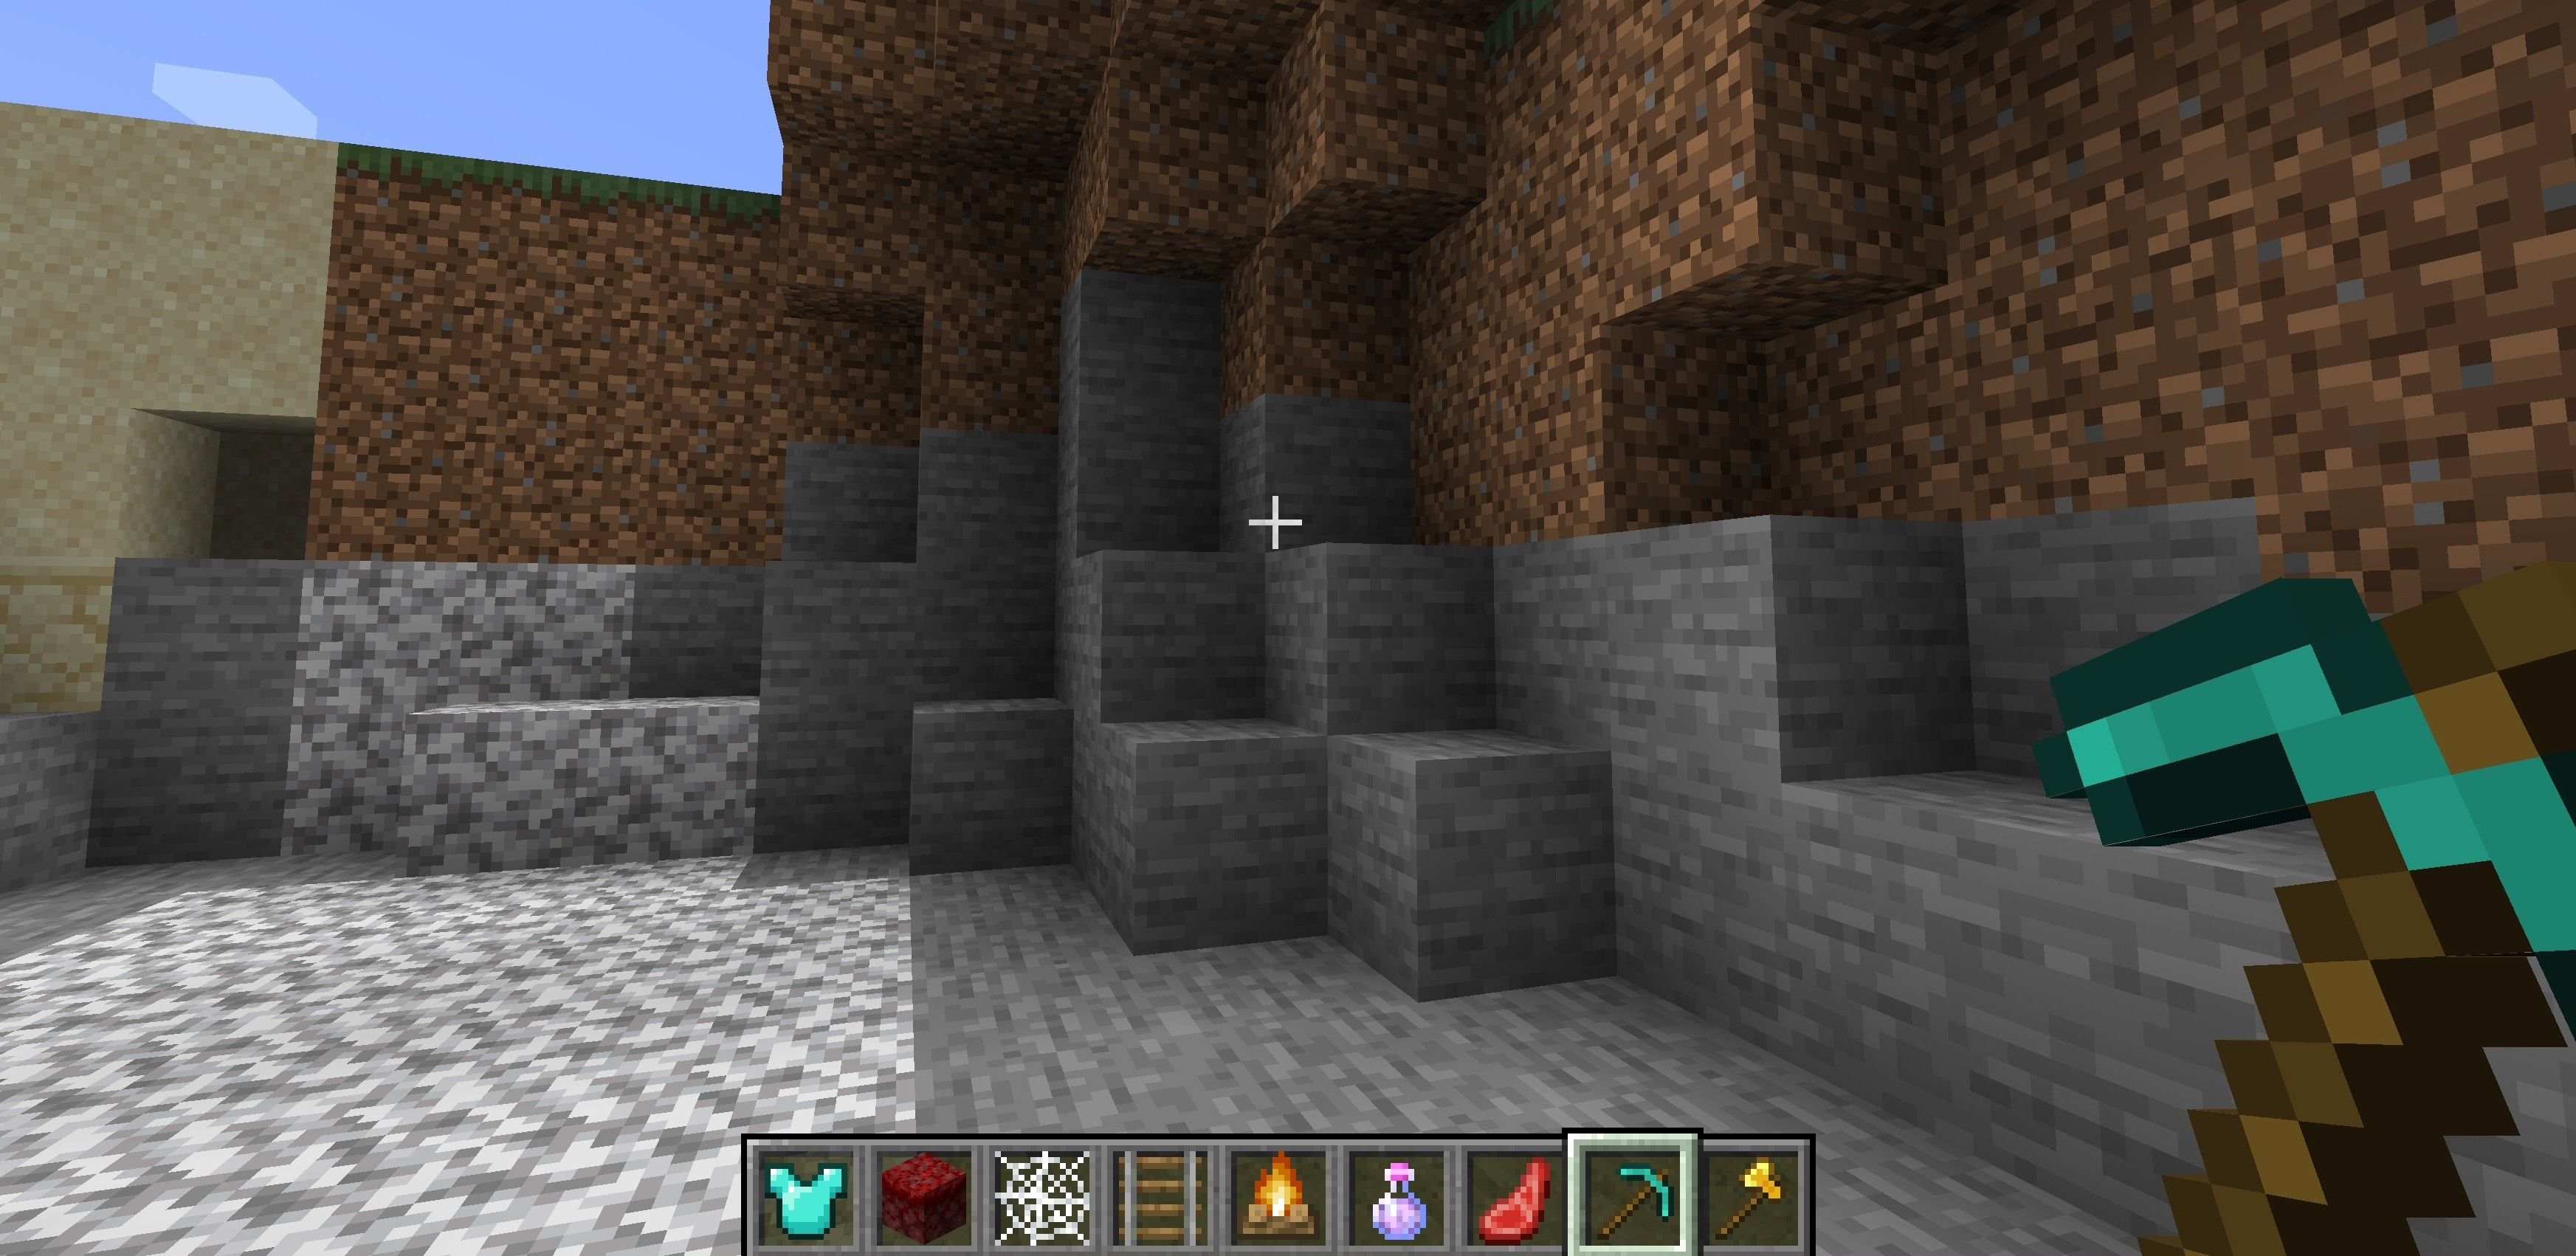
\includegraphics[width=8cm]{ressources/minecraft.jpg}
    \end{center}


\end{frame}
\begin{frame}
    \frametitle{}

    \begin{center}
        \framebox{Quel paradigme mettre en place pour programmer Minecraft?}
    \end{center}

\end{frame}
\section{Principes du jeu}
\begin{frame}
    \frametitle{Principes du jeu}

    \begin{center}
        \centering
        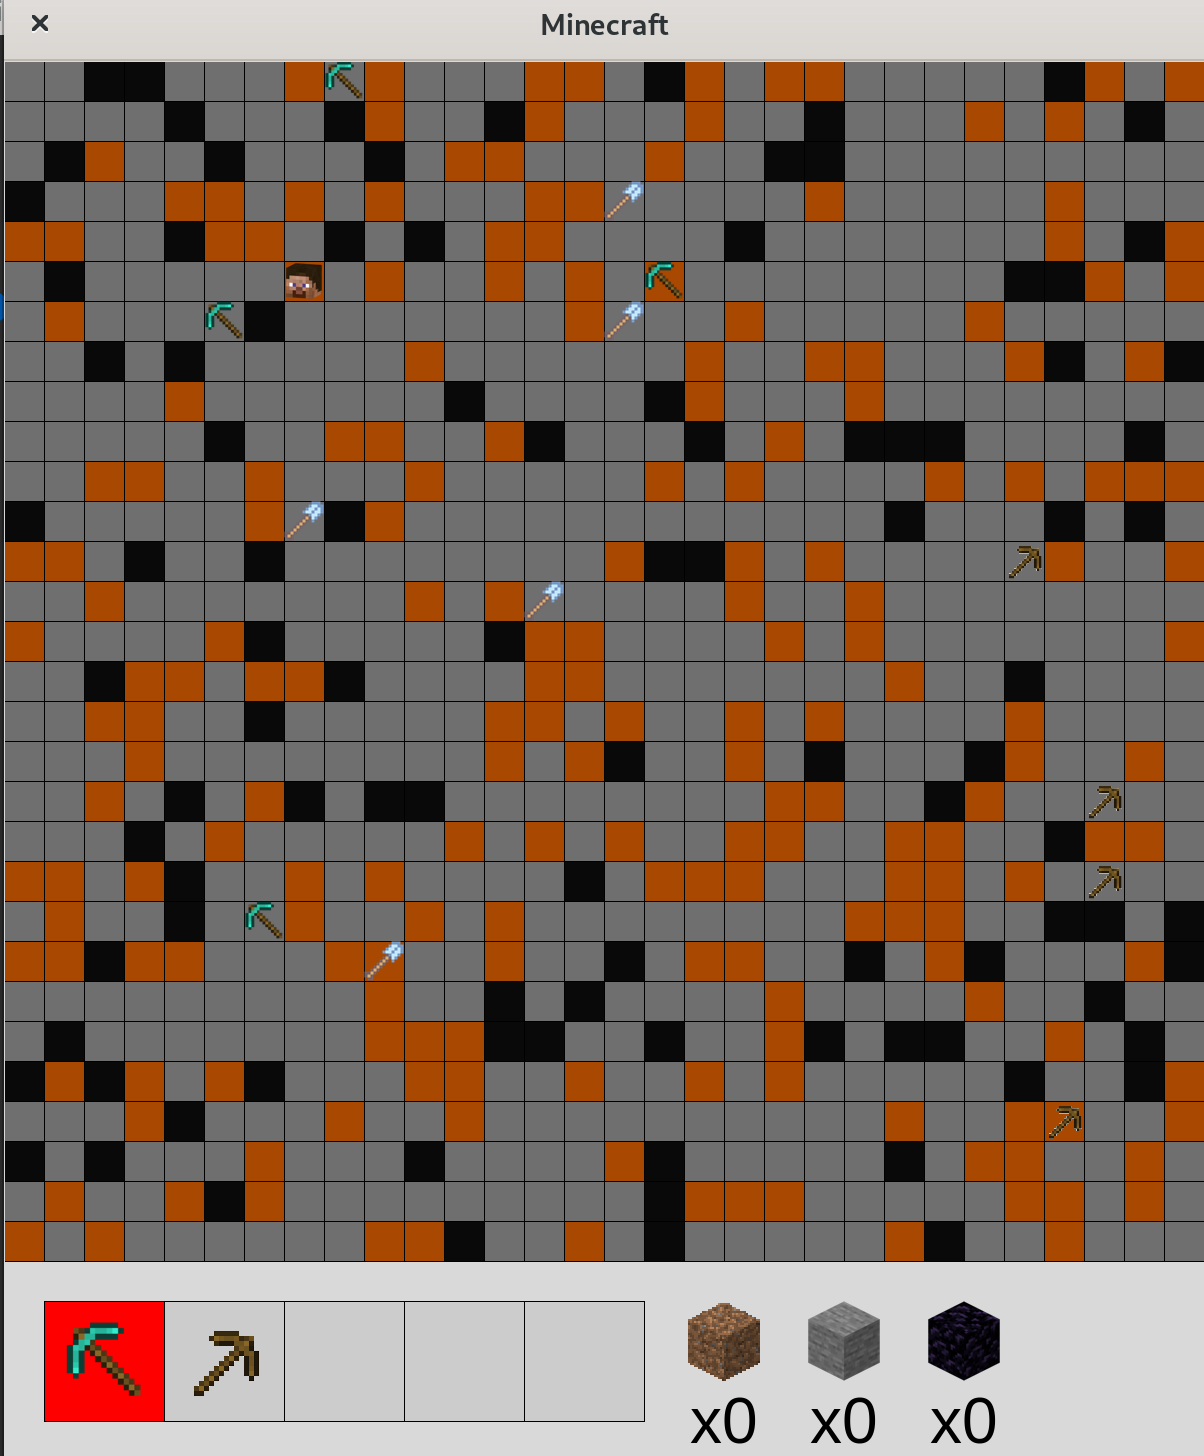
\includegraphics[width=6cm]{ressources/jeu.png}
        \captionof{figure}{Une version simplifiée}
        \label{jeu}
    \end{center}
\note{\fcolorbox{black}{red}{{\LARGE faire une démo}}}
\end{frame}
\begin{frame}
    \frametitle{Règles}

    \begin{itemize}
        \item R: ramasser un outil,
        \item W X C V B: choisir un outil de l'inventaire,
        \item Espace: miner,
        \item Flèches: se déplacer.
    \end{itemize}

    Le moteur du jeu se chargera de l'affichage graphique des concepts présentés ci-après.
\end{frame}
\begin{frame}
    \frametitle{3 types de blocs}

    \begin{center}
        \begin{tabular}{ccc}
            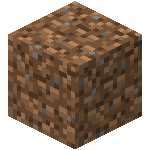
\includegraphics[width=3cm]{ressources/terre.png} &
            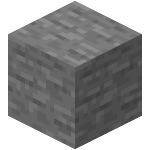
\includegraphics[width=3cm]{ressources/roche.png} &
            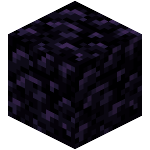
\includegraphics[width=3cm]{ressources/obsidienne.png}                 \\
            terre                                             & roche & obsidienne \\
        \end{tabular}
        \captionof{figure}{Des caractéristiques différentes}
    \end{center}

\end{frame}
\begin{frame}
    \frametitle{3 types d'outils}

    \begin{center}
        \begin{tabular}{ccc}
            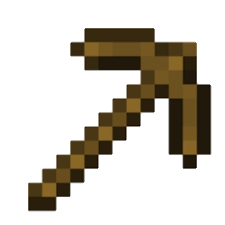
\includegraphics[width=3cm]{ressources/wood_pickaxe.png}    &
            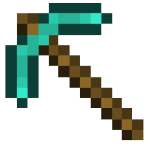
\includegraphics[width=3cm]{ressources/diamond_pickaxe.png} &
            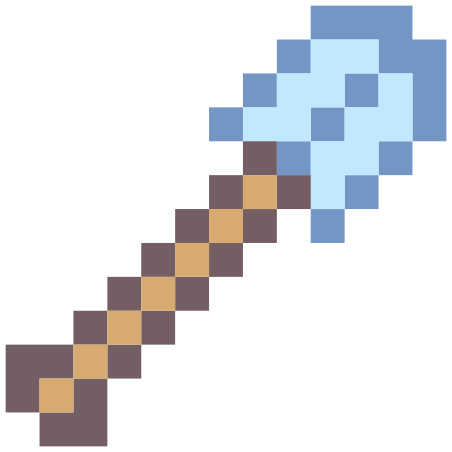
\includegraphics[width=3cm]{ressources/shovel.png}                                      \\
            pioche en bois                                              & pioche en diamant & pelle \\
        \end{tabular}
        \captionof{figure}{Des actions différentes}
    \end{center}

\end{frame}
\begin{frame}
    \frametitle{Un héros avec des capacités}

    \begin{center}
        \begin{tabular}{cp{0.5\textwidth}}
            
\includegraphics[width=3cm]{ressources/head.png} &
            \begin{itemize}
                \item récupérer des outils,
                \item stocker des blocs,
                \item miner des blocs,
                \item labourer des terres.
            \end{itemize}                          \\
        \end{tabular}
    \end{center}

\end{frame}
\section{Programmation orientée objet}
\subsection{Définition}
\begin{frame}
    \frametitle{Définition}

    Le \textbf{paradigme objet} consiste à construire des \emph{objets} et les faire interagir entre eux. Un objet représente une entité physique, un concept\dots  

\end{frame}
\begin{frame}
    \frametitle{}

    Un objet possède:
    \begin{itemize}
        \item des caractéristiques: \textbf{les attributs},
        \item des capacités: \textbf{les méthodes}.
    \end{itemize}

\end{frame}
\begin{frame}
    \frametitle{Exemple
    }

    Une voiture:
    \begin{itemize}
        \item attributs: rouge, électrique\dots
        \item méthodes: rouler, freiner\dots
    \end{itemize}

\end{frame}
\subsection{Modélisation}
\begin{frame}
    \frametitle{Modélisation}

    Il est nécessaire de modéliser le problème en représentant les objets et leurs interactions.

\end{frame}
\begin{frame}
    \frametitle{Les blocs et leurs attributs}


        \begin{center}
            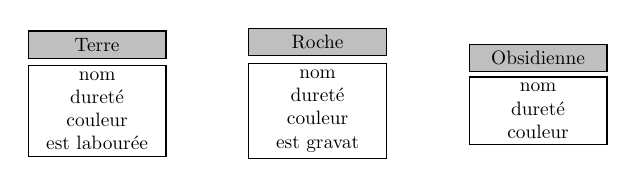
\begin{tikzpicture}[every text node part/.style={align=center},scale=0.7, transform shape]
                \node[draw,fill=gray!50,minimum width=2.5cm, minimum height=0.5cm] (terre) at (0,1.2) {Terre};
                \node[draw,minimum width=2.5cm] at (0,0) {nom \\ dureté \\ couleur \\ est labourée};

                \node[draw,fill=gray!50,minimum width=2.5cm, minimum height=0.5cm] (roche) at (4,1.25) {Roche};
                \node[draw,minimum width=2.5cm] at (4,0) {nom \\ dureté \\ couleur \\ est gravat};

                \node[draw,fill=gray!50,minimum width=2.5cm, minimum height=0.5cm] (obsidienne) at (8,0.96) {Obsidienne};
                \node[draw,minimum width=2.5cm] at (8,0) {nom \\ dureté \\ couleur};
            \end{tikzpicture}
        \end{center}


\end{frame}
\begin{frame}
    \frametitle{Les outils et leurs méthodes}

        \begin{center}
            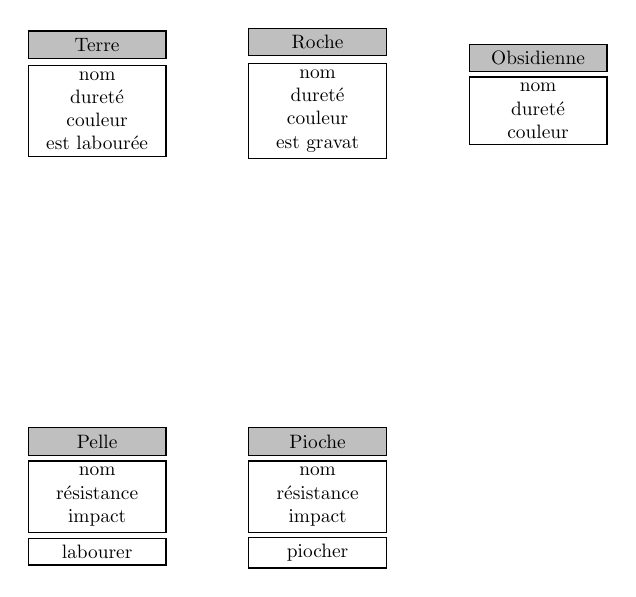
\begin{tikzpicture}[every text node part/.style={align=center},scale=0.7, transform shape]
                \node[draw,fill=gray!50,minimum width=2.5cm, minimum height=0.5cm] (terre) at (0,1.2) {Terre};
                \node[draw,minimum width=2.5cm] at (0,0) {nom \\ dureté \\ couleur \\ est labourée};

                \node[draw,fill=gray!50,minimum width=2.5cm, minimum height=0.5cm] (roche) at (4,1.25) {Roche};
                \node[draw,minimum width=2.5cm] at (4,0) {nom \\ dureté \\ couleur \\ est gravat};

                \node[draw,fill=gray!50,minimum width=2.5cm, minimum height=0.5cm] (obsidienne) at (8,0.96) {Obsidienne};
                \node[draw,minimum width=2.5cm] at (8,0) {nom \\ dureté \\ couleur};


                \node[draw,fill=gray!50,minimum width=2.5cm, minimum height=0.5cm] (pelle) at (0,-6) {Pelle};
                \node[draw,minimum width=2.5cm] at (0,-7) {nom \\ résistance \\ impact};
                \node[draw,minimum width=2.5cm] at (0,-8) {labourer};


                \node[draw,fill=gray!50,minimum width=2.5cm, minimum height=0.5cm] (pioche) at (4,-6) {Pioche};
                \node[draw,minimum width=2.5cm] at (4,-7) {nom \\ résistance \\ impact};
                \node[draw,minimum width=2.5cm] at (4,-8.02) {piocher};

            \end{tikzpicture}
        \end{center}


\end{frame}
\begin{frame}
    \frametitle{Le joueur et les relations}


        \begin{center}
            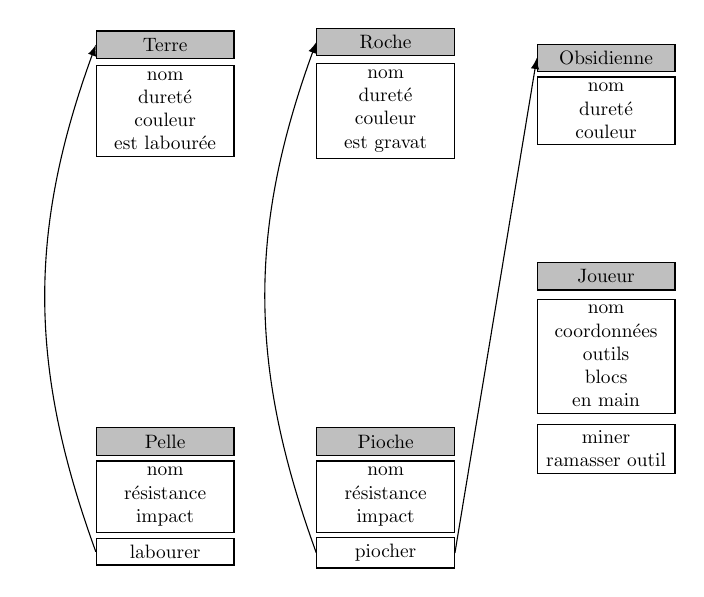
\begin{tikzpicture}[every text node part/.style={align=center},scale=0.7, transform shape]
                \node[draw,fill=gray!50,minimum width=2.5cm, minimum height=0.5cm] (terre) at (0,1.2) {Terre};
                \node[draw,minimum width=2.5cm] at (0,0) {nom \\ dureté \\ couleur \\ est labourée};

                \node[draw,fill=gray!50,minimum width=2.5cm, minimum height=0.5cm] (roche) at (4,1.25) {Roche};
                \node[draw,minimum width=2.5cm] at (4,0) {nom \\ dureté \\ couleur \\ est gravat};

                \node[draw,fill=gray!50,minimum width=2.5cm, minimum height=0.5cm] (obsidienne) at (8,0.96) {Obsidienne};
                \node[draw,minimum width=2.5cm] at (8,0) {nom \\ dureté \\ couleur};


                \node[draw,fill=gray!50,minimum width=2.5cm, minimum height=0.5cm] (pelle) at (0,-6) {Pelle};
                \node[draw,minimum width=2.5cm] at (0,-7) {nom \\ résistance \\ impact};
                \node[draw,minimum width=2.5cm] (labourer) at (0,-8) {labourer};


                \node[draw,fill=gray!50,minimum width=2.5cm, minimum height=0.5cm] (pioche) at (4,-6) {Pioche};
                \node[draw,minimum width=2.5cm] at (4,-7) {nom \\ résistance \\ impact};
                \node[draw,minimum width=2.5cm] (piocher) at (4,-8.02) {piocher};


                \node[draw,fill=gray!50,minimum width=2.5cm, minimum height=0.5cm] (joueur) at (8,-3) {Joueur};
                \node[draw,minimum width=2.5cm] at (8,-4.45) {nom \\ coordonnées \\ outils \\ blocs \\ en main};
                \node[draw,minimum width=2.5cm] at (8,-6.13) {miner \\ ramasser outil};

                \draw[->,>=latex] (labourer.west) to[bend left=20] (terre.west);
                \draw[->,>=latex] (piocher.west) to[bend left=20] (roche.west);
                \draw[->,>=latex] (piocher.east) to (obsidienne.west);

            \end{tikzpicture}
        \end{center}

    \note[item]{faire relations avec joueur à la main}
    \note[item]{ramasser outil vers les outils}
    \note[item]{miner vers les blocs}
\end{frame}
\subsection{Instances d'un objet}
\begin{frame}
    \frametitle{Instances d'un objet}

    \begin{itemize}
        \item<1->Chaque objet est un modèle qui peut être vu comme un squelette.
        \begin{center}
            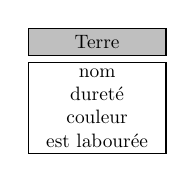
\begin{tikzpicture}[every text node part/.style={align=center},scale=0.7, transform shape]
                \node[draw,fill=gray!50,minimum width=2.5cm, minimum height=0.5cm] (terre) at (0,1.2) {Terre};
                \node[draw,minimum width=2.5cm] at (0,0) {nom \\ dureté\\ couleur\\ est labourée};
            \end{tikzpicture}
        \end{center}
        \item<2->On crée une \textbf{instance} de l'objet. C'est cette instance qui interagit dans le programme.
              \begin{center}
                  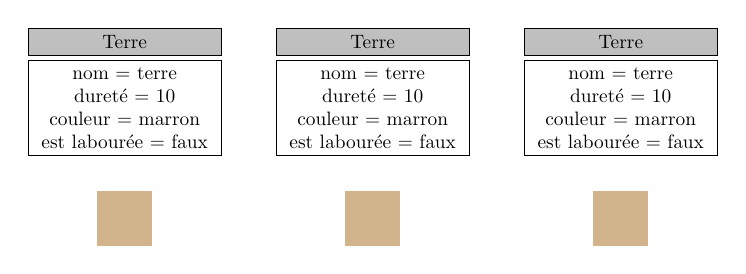
\begin{tikzpicture}[every text node part/.style={align=center},scale=0.7, transform shape]
                      \node[draw,fill=gray!50,minimum width=3.5cm, minimum height=0.5cm] (terre) at (0,1.2) {Terre};
                      \node[draw,minimum width=3.5cm] at (0,0) {nom = terre \\ dureté = 10\\ couleur = marron\\ est labourée = faux};
                      \node[draw,fill=gray!50,minimum width=3.5cm, minimum height=0.5cm] (terre) at (4.5,1.2) {Terre};
                      \node[draw,minimum width=3.5cm] at (4.5,0) {nom = terre \\ dureté = 10\\ couleur = marron\\ est labourée = faux};
                      \node[draw,fill=gray!50,minimum width=3.5cm, minimum height=0.5cm] (terre) at (9,1.2) {Terre};
                      \node[draw,minimum width=3.5cm] at (9,0) {nom = terre \\ dureté = 10\\ couleur = marron\\ est labourée = faux};
                      \fill [color=Tan] (-0.5,-2.5) -- (0.5,-2.5) -- (0.5,-1.5) -- (-0.5,-1.5) -- cycle;
                      \fill [color=Tan] (4,-2.5) -- (5,-2.5) -- (5,-1.5) -- (4,-1.5) -- cycle;
                      \fill [color=Tan] (8.5,-2.5) -- (9.5,-2.5) -- (9.5,-1.5) -- (8.5,-1.5) -- cycle;
                  \end{tikzpicture}
              \end{center}
        
    \end{itemize}

\end{frame}
\begin{frame}
    \begin{itemize}
        \item On crée une \textbf{instance} de l'objet. C'est cette instance qui interagit dans le programme.
              \begin{center}
                  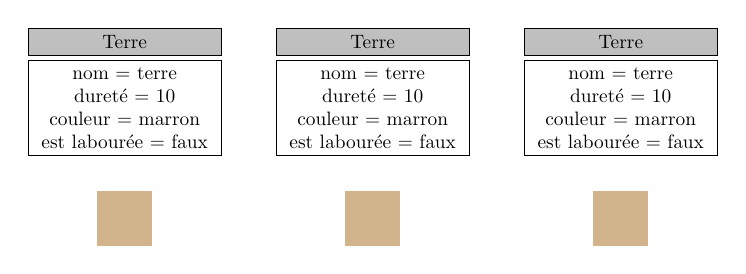
\begin{tikzpicture}[every text node part/.style={align=center},scale=0.7, transform shape]
                      \node[draw,fill=gray!50,minimum width=3.5cm, minimum height=0.5cm] (terre) at (0,1.2) {Terre};
                      \node[draw,minimum width=3.5cm] at (0,0) {nom = terre \\ dureté = 10\\ couleur = marron\\ est labourée = faux};
                      \node[draw,fill=gray!50,minimum width=3.5cm, minimum height=0.5cm] (terre) at (4.5,1.2) {Terre};
                      \node[draw,minimum width=3.5cm] at (4.5,0) {nom = terre \\ dureté = 10\\ couleur = marron\\ est labourée = faux};
                      \node[draw,fill=gray!50,minimum width=3.5cm, minimum height=0.5cm] (terre) at (9,1.2) {Terre};
                      \node[draw,minimum width=3.5cm] at (9,0) {nom = terre \\ dureté = 10\\ couleur = marron\\ est labourée = faux};
                      \fill [color=Tan] (-0.5,-2.5) -- (0.5,-2.5) -- (0.5,-1.5) -- (-0.5,-1.5) -- cycle;
                      \fill [color=Tan] (4,-2.5) -- (5,-2.5) -- (5,-1.5) -- (4,-1.5) -- cycle;
                      \fill [color=Tan] (8.5,-2.5) -- (9.5,-2.5) -- (9.5,-1.5) -- (8.5,-1.5) -- cycle;
                  \end{tikzpicture}
              \end{center}
        \item Chaque instance est indépendante des autres.
        \begin{center}
            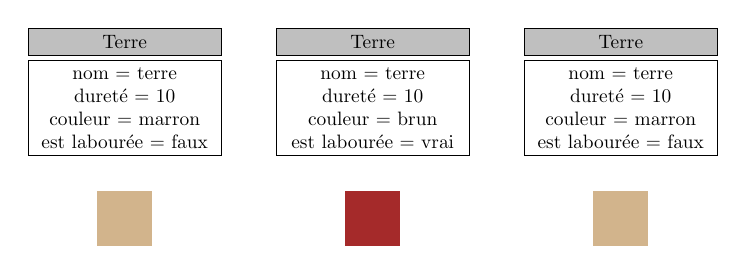
\begin{tikzpicture}[every text node part/.style={align=center},scale=0.7, transform shape]
                \node[draw,fill=gray!50,minimum width=3.5cm, minimum height=0.5cm] (terre) at (0,1.2) {Terre};
                \node[draw,minimum width=3.5cm] at (0,0) {nom = terre \\ dureté = 10\\ couleur = marron \\ est labourée = faux};
                \node[draw,fill=gray!50,minimum width=3.5cm, minimum height=0.5cm] (terre) at (4.5,1.2) {Terre};
                \node[draw,minimum width=3.5cm] at (4.5,0) {nom = terre \\ dureté = 10\\ couleur = brun \\ est labourée = vrai};
                \node[draw,fill=gray!50,minimum width=3.5cm, minimum height=0.5cm] (terre) at (9,1.2) {Terre};
                \node[draw,minimum width=3.5cm] at (9,0) {nom = terre \\ dureté = 10\\ couleur = marron\\ est labourée = faux};
                \fill [color=Tan] (-0.5,-2.5) -- (0.5,-2.5) -- (0.5,-1.5) -- (-0.5,-1.5) -- cycle;
                \fill [color=Brown] (4,-2.5) -- (5,-2.5) -- (5,-1.5) -- (4,-1.5) -- cycle;
                \fill [color=Tan] (8.5,-2.5) -- (9.5,-2.5) -- (9.5,-1.5) -- (8.5,-1.5) -- cycle;
            \end{tikzpicture}
        \end{center}
    \end{itemize}

\end{frame}

\section{Implémentation}
\subsection{Créer un objet}
\begin{frame}[fragile]
    \frametitle{Créer un objet}

    \begin{center}
    \begin{lstlisting}[language=Python , basicstyle=\small, xleftmargin=2em, xrightmargin=2em]
class Terre
\end{lstlisting}
    \captionof{code}{Le mot-clé \textbf{\texttt{class}}}

    \end{center}

\end{frame}
\subsection{Initialiser les attributs}
\begin{frame}[fragile]
    \frametitle{Initialiser les attributs}

La \emph{méthode} \texttt{\textbf{\_\_init\_\_}} est appelée automatiquement quand nous instancions un objet.
\begin{center}
\begin{lstlisting}[language=Python , basicstyle=\small, xleftmargin=2em, xrightmargin=2em]
class Terre:
    def __init__(self):
        self.nom = "terre"
        self.durete = 10
        self.couleur = "#a94800"
        self.est_labouree = False
\end{lstlisting}
\captionof{code}{Les attributs sont initialisés dans le \emph{constructeur}.}
\label{CODE}
\end{center}

\end{frame}
\begin{frame}
    \frametitle{}

    Le mot-clé \textbf{\texttt{self}} identifie l'instance de l'objet.

\end{frame}
\begin{frame}
    \frametitle{}

    \begin{activite}
    \begin{enumerate}
        \item Télécharger et extraire le dossier compressé \textbf{minecraft.zip} sur le site \url{https://cviroulaud.github.io}
        \item Dans le fichier \textbf{blocs.py} construire les objets:
        \begin{center}
            \begin{tabular}{*{2}{p{0.5\textwidth}}}
            \textbf{\texttt{Roche}}
            \begin{itemize}
                \item nom: stone,
                \item durete: 100,
                \item couleur: \#6f6f6f,
                \item est\_gravat: False
            \end{itemize}&
            \textbf{\texttt{Obsidienne}}
            \begin{itemize}
                \item nom: obsidian,
                \item durete: 1000,
                \item couleur: \#090909
            \end{itemize}\\
            \end{tabular}
        \end{center}
    \end{enumerate}
    \end{activite}

\end{frame}
\begin{frame}[fragile]
    \frametitle{Correction}

\begin{center}
\begin{lstlisting}[language=Python , basicstyle=\small, xleftmargin=2em, xrightmargin=2em]
class Roche:
    def __init__(self):
        self.nom = "stone"
        self.durete = 100
        self.couleur = "#6f6f6f"
        self.est_gravat = False


class Obsidienne:
    def __init__(self):
        self.nom = "obsidian"
        self.durete = 1000
        self.couleur = "#090909"
\end{lstlisting}
\end{center}    

\end{frame}
\begin{frame}[fragile]
    \frametitle{}    
    \begin{center}
    \begin{lstlisting}[language=Python , basicstyle=\small, xleftmargin=2em, xrightmargin=2em]
class Pioche:
    def __init__(self, nom: str):
        self.nom = nom
        if nom == "wood_pickaxe":
            self.resistance = 30
            self.impact = 5
        elif nom == "diamond_pickaxe":
            self.resistance = 100
            self.impact = 100
\end{lstlisting}
    \captionof{code}{Une autre classe: il est possible d'ajouter des paramètres au constructeur.}
    \label{CODE}
    \end{center}
\note{une autre approche: un même objet pour toutes les pioches.}
\end{frame}
\subsection{Définir les méthodes}
\begin{frame}
    \frametitle{Définir les méthodes}

    On appelle \textbf{méthode} une fonction interne à la classe de l'objet. 

    En Python, le premier paramètre est \textbf{toujours} \textbf{\texttt{self}}. C'est un attribut \textbf{interne} à la classe.
\note{en javascript c'est \textbf{this}}
\end{frame}
\begin{frame}[fragile]
    \frametitle{}

    \begin{center}
    \begin{lstlisting}[language=Python , basicstyle=\small, xleftmargin=2em, xrightmargin=2em]
def piocher(self, bloc: object) -> bool:
    """
    donne un coup sur le bloc

    Args:
        bloc (object): le bloc miné

    Returns:
        bool: False si l'outil est complètement usé
    """
\end{lstlisting}
    \captionof{code}{Signature de la méthode de la classe \textbf{\texttt{Pioche}}}
    \label{CODE}
    \end{center}

\end{frame}
\begin{frame}[fragile]
    \frametitle{}

    \begin{center}
    \begin{lstlisting}[language=Python , basicstyle=\small, xleftmargin=2em, xrightmargin=2em]
def piocher(self, bloc: object) -> bool:
    """
    donne un coup sur le bloc

    Args:
        bloc (object): le bloc miné

    Returns:
        bool: False si l'outil est complètement usé
    """
    bloc.durete -= self.impact
\end{lstlisting}
    \captionof{code}{On accède à un attribut \textbf{par la structure à \emph{point}}.}
    \label{CODE}
    \end{center}

\end{frame}
\begin{frame}[fragile]
    \frametitle{}

    \begin{itemize}
        \item<1-> En Python, les attributs et les méthodes sont publics. Ils sont accessibles de n'importe quel endroit du programme.
        \begin{center}
        \begin{lstlisting}[language=Python , basicstyle=\small, xleftmargin=2em, xrightmargin=2em]
bloc.durete
\end{lstlisting}
        \end{center}
        \item<2->Les attributs et méthodes \emph{internes} à la classe sont accessibles avec le mot-clé \textbf{\texttt{self}}.
        \begin{center}
        \begin{lstlisting}[language=Python , basicstyle=\small, xleftmargin=2em, xrightmargin=2em]
self.impact
\end{lstlisting}
        \end{center}
    \end{itemize}

\end{frame}
\begin{frame}[fragile]
    \frametitle{}

    \begin{center}
    \begin{lstlisting}[language=Python , basicstyle=\small, xleftmargin=2em, xrightmargin=2em]
def piocher(self, bloc: object) -> bool:
    """
    donne un coup sur le bloc

    Args:
        bloc (object): le bloc miné

    Returns:
        bool: False si l'outil est complètement usé
    """
    bloc.durete -= self.impact
    self.resistance -= USURE
    if self.resistance <= 0:
        return False
    return True
\end{lstlisting}
    \captionof{code}{Méthode de la classe \textbf{\texttt{Pioche}}}
    \label{CODE}
    \end{center}

\end{frame}
\begin{frame}
    \frametitle{}

    \begin{activite}
    Dans le fichier \textbf{outils.py}, construire la méthode \textbf{\texttt{labourer}} de la classe \textbf{\texttt{Pelle}}.
    \begin{itemize}
        \item S'aider de la \emph{docstring}.
        \item La couleur labourée est \#712712.
        \item La pelle s'use.
    \end{itemize}
    \end{activite}

\end{frame}
\begin{frame}[fragile]
    \frametitle{Correction}

\begin{center}
\begin{lstlisting}[language=Python , basicstyle=\small, xleftmargin=2em, xrightmargin=2em]
def labourer(self, bloc: object) -> bool:
    """
    laboure un bloc terre (non déjà labourée), 
    ne fait rien sinon

    Args:
        bloc (object): le bloc en cours

    Returns:
        bool: False si l'outil est complètement usé
    """
    if bloc.nom == "dirt" and not bloc.est_labouree:
        bloc.est_labouree = True
        bloc.couleur = "#712712"
        self.resistance -= USURE
        if self.resistance <= 0:
            return False
    return True
\end{lstlisting}
\end{center}

\end{frame}
\begin{frame}[fragile]
    \frametitle{Étude de la classe Joueur}

    \begin{center}
    \begin{lstlisting}[language=Python , basicstyle=\small, xleftmargin=2em, xrightmargin=2em]
class Joueur:
    def __init__(self, n: str):
        self.nom = n
        self.x = 0
        self.y = 0
        self.outils = []  # 5 maxi
        self.blocs = {"dirt": 0, "stone": 0, "obsidian": 0}
        self.en_main = 0  # outil en main
\end{lstlisting}
    \captionof{code}{Constructeur}
    \label{CODE}
    \end{center}
\note{inventaires: une liste et un dict}
\end{frame}
\begin{frame}[fragile]
    \frametitle{Des méthodes}

\begin{center}
\begin{lstlisting}[language=Python , basicstyle=\small, xleftmargin=2em, xrightmargin=2em]
def miner(self, bloc: object) -> bool:
    """
    donne un coup sur le bloc avec l'outil en cours
    ou la main

    Args:
        bloc (object): le bloc miné

    Returns:
        bool: True si le bloc est complètement miné
    """
\end{lstlisting}
\captionof{code}{miner}
\label{CODE}
\end{center}

\end{frame}
\begin{frame}[fragile]
    \frametitle{}

    \begin{center}
    \begin{lstlisting}[language=Python , basicstyle=\small, xleftmargin=2em, xrightmargin=2em]
def ramasser_outil(self, outil: object) -> bool:
    """
    place l'outil dans l'inventaire s'il y a de la place

    Args:
        outil (object): l'outil ramassé

    Returns:
        bool: True si l'outil a été ramassé
    """
\end{lstlisting}
    \captionof{code}{ramasser}
    \label{CODE}
    \end{center}

\end{frame}
\begin{frame}
    \frametitle{}

    \begin{activite}
    Compléter les méthodes de la classe \textbf{\texttt{Joueur}} dans le fichier \textbf{joueur.py}
    \end{activite}

\end{frame}
\begin{frame}[fragile]
    \frametitle{Correction}

    \begin{center}
    \begin{lstlisting}[language=Python , basicstyle=\small, xleftmargin=2em, xrightmargin=2em]
# récupère l'impact de l'outil en cours
impact = self.outils[self.en_main].impact
# l'outil s'use
self.outils[self.en_main].resistance -= USURE
\end{lstlisting}
    \captionof{code}{Méthode \textbf{\texttt{miner}}}
    \label{CODE}
    \end{center}
\begin{itemize}
    \item \textbf{\texttt{impact}} est une variable \emph{locale} à la méthode.
    \item \textbf{\texttt{USURE}} est une variable globale au programme.
    \item \textbf{\texttt{self.outils}} est un attribut de la classe.
    \item \textbf{\texttt{self.outils[self.en\_main]}} fait référence à un objet (un outil).
\end{itemize}
\end{frame}
\begin{frame}[fragile]
    \frametitle{Correction}

    \begin{center}
    \begin{lstlisting}[language=Python , basicstyle=\small, xleftmargin=2em, xrightmargin=2em]
if outil is not None:
    if len(self.outils) < NB_OUTILS_INVENTAIRE:
        # l'outil est ajouté à l'inventaire
        self.outils.append(outil)
        return True
return False
\end{lstlisting}
    \captionof{code}{Méthode \textbf{\texttt{ramasser\_outil}}}
    \label{CODE}
    \end{center}
\begin{itemize}
    \item \textbf{\texttt{outil}} est un paramètre de la méthode.
    \item \textbf{\texttt{self.outils}} est une méthode de la classe.
\end{itemize}
\end{frame}
\subsection{Instancier une classe}
\begin{frame}[fragile]
    \frametitle{Instancier une classe}

   Les classes vont permettre de créer les objets manipulables dans le programme.
   \begin{center}
   \begin{lstlisting}[language=Python , basicstyle=\small, xleftmargin=2em, xrightmargin=2em]
un_bloc_terre = Terre()
une_pioche_bois = Pioche("wood_pickaxe")
\end{lstlisting}
   \captionof{code}{Instanciations}
   \label{CODE}
   \end{center} 
\note{on trouve aussi \emph{instancier un objet}}
\end{frame}
\begin{frame}
    \frametitle{}
Le jeu crée 900 blocs (\textbf{\texttt{LARGEUR*HAUTEUR}}):
\begin{itemize}
    \item 100 blocs d'obsidienne,
    \item 200 blocs de terre,
    \item 600 blocs de roche.
\end{itemize}
Il place ensuite au hasard 15 outils:
\begin{itemize}
    \item 5 pelles,
    \item 5 pioches en bois,
    \item 5 pioches en diamant.
\end{itemize}
La classe \textbf{\texttt{Moteur}} fournit la méthode \textbf{\texttt{donnees\_coordonnees()}} qui renvoie un tuple (x,y) de coordonnées non encore utilisé.
    \begin{activite}
Compléter le fichier \textbf{minecraft.py} en s'aidant des informations ci-dessus.
    \end{activite}

\end{frame}
\begin{frame}[fragile]
    \frametitle{Correction}

    \begin{center}
    \begin{lstlisting}[language=Python , basicstyle=\small, xleftmargin=2em, xrightmargin=2em]
for i in range(0, 100):
    grille[i] = Obsidienne()
for i in range(100, 300):
    grille[i] = Terre()
for i in range(300, 900):
    grille[i] = Roche()   
\end{lstlisting}
    \captionof{code}{Créer les blocs}
    \label{CODE}
    \end{center}

\end{frame}
\begin{frame}
    \frametitle{Affichage}

    \begin{center}
    \centering
    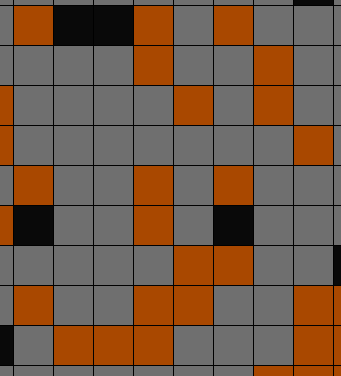
\includegraphics[width=5cm]{ressources/blocs.png}
    \captionof{figure}{Le moteur assurera la représentation graphique des objets.}
    \label{IMG}
    \end{center}

\end{frame}
\begin{frame}[fragile]
    \frametitle{Correction}

    \begin{center}
    \begin{lstlisting}[language=Python , basicstyle=\small, xleftmargin=1.8em, xrightmargin=2em]
for i in range(5):
    outils_poses[moteur.donner_coordonnees()] = Pioche("wood_pickaxe")
    outils_poses[moteur.donner_coordonnees()] = Pioche("diamond_pickaxe")
    outils_poses[moteur.donner_coordonnees()] = Pelle()
      
\end{lstlisting}
    \captionof{code}{Placer les outils}
    \label{CODE}
    \end{center}

\end{frame}
\begin{frame}
    \frametitle{}

    \begin{center}
    \centering
    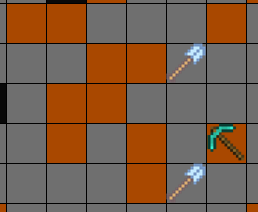
\includegraphics[width=5cm]{ressources/outils.png}
    \captionof{figure}{Le moteur s'occupera d'afficher les outils.}
    \label{IMG}
    \end{center}

\end{frame}
\begin{frame}
    \frametitle{Code complet}

    Le code complet est accessible \href{https://cviroulaud.github.io/terminale/langages/paradigmes/POO/minecraft/scripts/minecraft-corrige.zip}{ici}.

\end{frame}
\end{document}